\section{Microwave Absorbers}

In some of the experimental modules microwaves are used to drive transitions.
This radiation needs to be contained so it does not interfere with other parts
of the experiment. In order to do so, we considered covering the interior metal
surfaces of some of the vacuum chambers with absorbing materials. In the
following, I present several types of radiation-absorbing sheets, then evaluate
how effective this approach can be at localizing the radiation.

\subsection{Simple absorbers}

\paragraph{Thin-film absorber}

\begin{figure}[b]
   \centering
  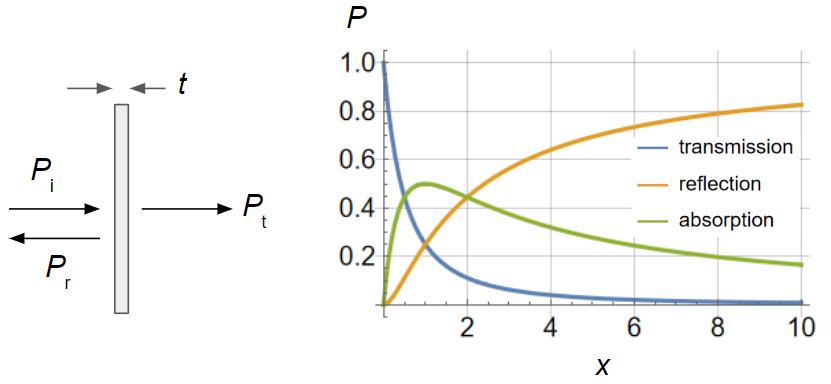
\includegraphics[width=.8\textwidth]{figs/todo/simplest.png}
    \caption[Thin-film absorber.]{Thin-film absorber. The plot shows the
    fraction of transmitted ($P_\text{t}$), reflected ($P_\text{r}$), and
    absorbed ($P_\text{a}$) power as a function of the parameter
    $x=Z_0t/(2\rho)$.}
  \label{simplest}
\end{figure}

In the simplest case, radiation is normally incident on an infinite resistive
sheet of resistivity $\rho$. In terms of the parameter $x=Z_0t/(2\rho)$, where
$Z_0\approx376.73\;\Omega$ is the impedance of free space, the fraction of power
transmitted, reflected, and absorbed is \cite[eqn~8.79]{goldsmith1998quasioptical}
%
\begin{align*}
   P_\text{t}=\frac{1}{(1+x)^2}
   ,\quad
   P_\text{r}=\frac{x^2}{(1+x)^2}
   ,\quad
   P_\text{a}=\frac{2x}{(1+x)^2}
   .
\end{align*}
%       
These expressions are plotted in Fig.~\ref{simplest}, where it is evident that
the resistive sheet can absorb at most half of the power when $x=1$, i.e.\ when
the sheet thickness is $t=2\rho/Z_0$. For gold
($\rho\approx2.4\cdot10^{-8}\;\Omega\cdot\text{m}$), this corresponds to a
thickness of $t\approx1\text{\AA}$, which would be thinner than a sheet a single
atom thick. In other words, this approach requires a material with a higher
resistivity, and even then offers only 3~dB of absorptive attenuation.

\paragraph{Two thin films between a substrate}

A much more flexible approach is to use two conductive (or resistive) sheets
separated by a dielectric substrate of refractive index $n$ and thickness $h$.
The resistivity of each sheet is given as ``ohms per square'', reflecting the
fact that the resistance between two opposite sides of a square piece of
material of a given thickness and bulk resistivity is independent of the size of
the square. The absorption of incident radiation (vacuum wavelength $\lambda_0$)
can be calculated with the usual Fabry--P\'erot methods and is
\cite{carli1981absorption}
%
\[
   A=\frac
   {4pq^2(f+f')+4pf(p+f'-q)(p+f'+q)\sin^2\beta}
   {q^2(2p+f+f')^2+(p+f-q)(p+f+q)(p+f+q)(f+f'-q)(p+f'+q)\sin^2\beta},
\]
%
where
%
\begin{align*}
   f            &= Z_0/R_\square = \text{reciprocal normalized surface resistance of left surface}\\
   f'           &= Z_0/R'_\square = \text{reciprocal normalized surface resistance of right surface}\\
   p            &= \cos\theta\\
   q            &= n\cos\theta_2\\
   \theta       &= \text{angle of incidence}\\
   \beta        &= (2\pi nh\cos\theta_2)/\lambda_0\\
   \cos\theta_2 &= 1-n^{-2}(1-\cos^2\theta).
\end{align*}
%
Perfect absorption ($A=1$) obtains in the case of the so-called ``Salisbury
screen', when one of the sheets has $F=Z_0/R_\square=1$ (nicknamed ``space
cloth'' since the resistivity equals the impedance of free space), while the
other is perfectly conductive ($f'=\infty$). The separation between the two
sheets needs to be
%
\[
   \beta=\frac{2\pi nh\cos\theta_2}{\lambda_0}=\frac{\pi}{2}
   \quad\to\quad
   h=\frac{\lambda_0}{4n}.
\]
%
At 26~GHz, the quarter wavelength is $\lambda_0/4\approx2.89$~mm, showing that
this approach could be implemented in practice. Fig.~\ref{salisbury} shows the
result for a HFSS simulation of a finite size absorber of this type; note how
the absorption as a function of sheet spacing shows a decaying sinusoidal
pattern. (An infinite-sized absorber, as simulated using periodic boundary
conditions, would not exhibit the decay.)

\begin{figure}
   \centering
  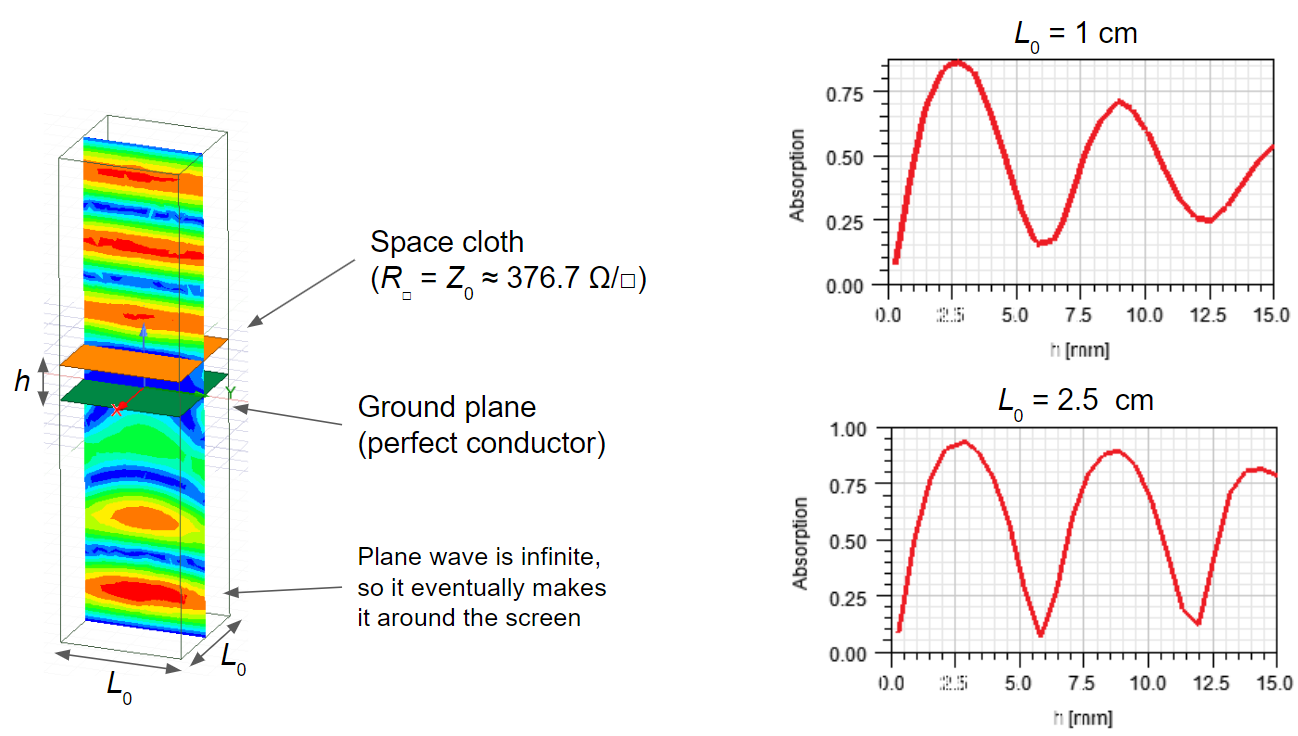
\includegraphics[width=\textwidth]{figs/todo/salisbury.png}
    \caption[Salisbury screen.]{Microwaves incident onto a finite-sized
    ``Salisbury screen'', showing the dependence of absorption as a function of
    separation between the perfect conductor and the ``space cloth'' of
    precisely tuned sheet resistivity. Note how the larger sample shows less of
    a decay of the sinusoid in the absorption plot; and infinite sheet would be
    perfectly sinusoidal.}
  \label{salisbury}
\end{figure}

Unlike the single-sheet absorber considered previously, the Salisbury screen is
frequency selective as would be expected for a Fabry--P\'erot structure. In
general, we expect the transmission or absorption to be periodic in wavelength
or cavity length. The periodicity has a length scale known as the free spectral
range. Between two spectral peaks, or between zero (say, in cavity length) and
the and the first peak, there are no additional peaks. In other words, no
resonance occurs if the cavity (or spacing between the two sheets) is much
shorter than the wavelength of the incident radiation.

For Fabry--P\'erot absorbers (or cavities in general), the spectral features
have a width determined by the reflectivity of the two mirrors, as characterized
by the finesse $F=\pi\sqrt{R}/(1-R)$, where $R=\sqrt{R_1R_2}$ is the geometric
mean of the two reflectivities. In the case of the Salisbury screen, we may
assume
%
\begin{align*}
   R_1&=\text{approx.\ 1 to 10, depending on $n$}\\
   R_2&=\text{1, i.e.\ a perfect metallic mirror}.
\end{align*}
%
Since one of the ``mirrors'' is determined by the air--substrate interface, it
has a poor reflectivity, which limits the finesse of the cavity to some small
number. Low-finesse cavities have very broad peaks, so there is some frequency
dependence even for ultra-short cavities.

The two-sheet absorber follows the Fabry--P\'erot theory. In the following
paragraph, we consider a very different approach to constructing
radiation-absorbing sheets which relies on resonances within planar structures
rather than cavity-type resonances.

\subsection{Metamaterial absorbers}

In a typical microwave metamaterial absorber (see Fig.~\ref{MA} for examples), a
simple pattern (typically, circles, crosses, lines, rectangles) is repeated many
times on a printed circuit board. On the absorption spectrum, the peaks are
typically very sharp. To achieve effective absorption at several frequencies,
the designers can choose patterns with several length scales (such as several
nested rings \cite{shen2012triple}, where the dimensions of each ring can be
tuned to match one of the frequencies of interest). For a broadband absorber,
patterns need to have a range of different length scales such that each
feature's absorption spectrum partially overlaps with another, slightly bigger
or smaller, feature (see \cite{yu2019broadband} for a good review of the topic).
In the following, I will discuss three ways of looking at metamaterial
absorbers: as Fabry--P\'erot resonators, as microstrip resonators, and as a
phased antenna array.

\begin{figure}
   \centering
  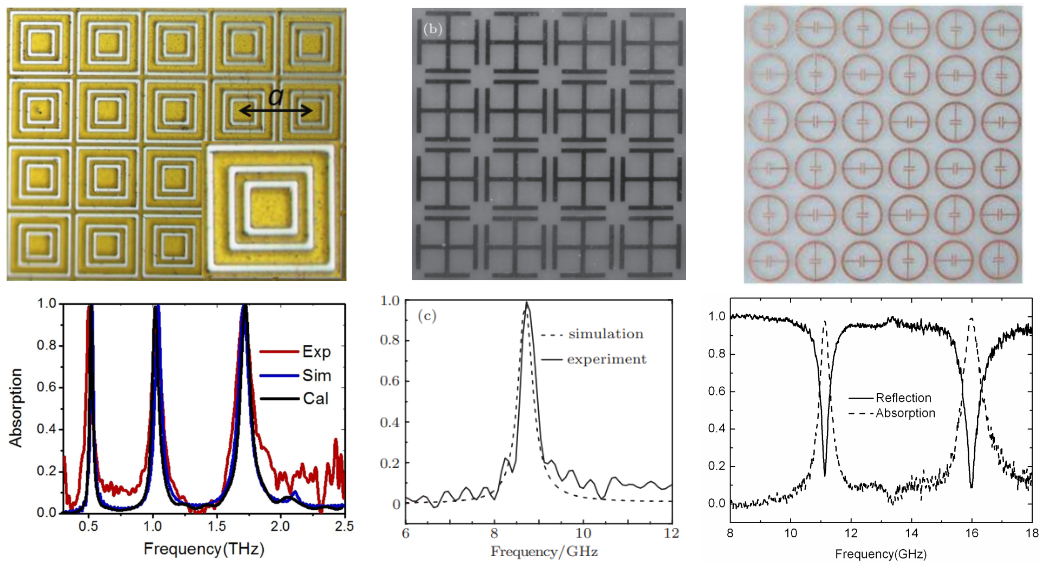
\includegraphics[width=\textwidth]{figs/todo/MA.png}
   \caption[Metamaterial absorber patterns and spectra.]{Examples of metamaterial absorber patterns (not to scale) with their
   corresponding absorption spectra. Figures taken from, respectively:
   \cite{shen2012triple}, \cite{wang2013multi}, \cite{li2010perfect}}
  \label{MA}
\end{figure}

\paragraph{Fabry--P\'erot theory}

A metamaterial absorber consists of a ground plane (assumed perfectly
conductive), a substrate, and a patterned surface. It is thus very similar to
the two-sheet absorbers considered in the previous section, such as the
Salisbury screen, except that the patterned surface itself has a
complicated frequency dependence. Applying the standard Fabry--P\'erot approach,
which they call ``multi-reflection interference theory'', Chen et al.
\cite{chen2012interference} obtain the reflection coefficient for a metamaterial
absorber,
%
\[
   \tilde{r}=\tilde{r}_{12}-\frac{\tilde{t}_{12}\tilde{t}_{21}e^{i2\tilde{\beta}}}{1+\tilde{r}_{21}e^{i2\tilde{\beta}}},
\]
%
where
$\tilde{r}_{12},\tilde{r}_{21},\tilde{t}_{12},\tilde{t}_{21},\tilde{\beta}$ are
numerically calculated and highly frequency dependent. While the authors
advertise their ``profound understanding of the underlying physics'' in coming
up with a theory that ``explains all features observed in narrowband
metamaterial absorbers'', the `profound physics' actually takes place in the
numerically calculated coefficients which encode the resonances that take place
within the patterned surface rather than the substrate-filled cavity formed by
the patterned surface and the ground plane.

From their simulations, the authors show a plot of absorption spectrum as a
function of the cavity length, where the resonant frequency changes by approx.\
20\%\ despite scanning the cavity length by a factor of 4, providing further
clues as to the inner workings of a metamaterial absorber. In the following, I
will show what I consider more enlightening ways to understand the underlying
physics.

\paragraph{Microstrip resonators}

A microstrip transmission line consists of a conductor of width $W$ placed over
a ground plane separated by a substrate of permittivity $\epsilon_\text{r}$ and
thickness $d$. The characteristic impedance of such a transmission line depends
on the dimensions of the conductor (specifically, the ratio of the width of the
line to the substrate height):
%
\[
   Z_0=\begin{dcases*}
      \frac{60}{\sqrt{\epsilon_\text{e}}}\ln\left(\frac{8d}{W}+\frac{W}{4d}\right)&\quad for $W/d\leq1$\\
      \frac{120\pi}{\sqrt{\epsilon_\text{e}}[W/d+1.393+0.667\ln(W/d+1.444)]}&\quad
      for $W/d\geq1$,
      \end{dcases*}
\]
%
where $\epsilon_\text{e}$ is the effective permittivity, which also depends on
the dimensions of the transmission line \cite[eqns~3.195--6]{pozar2006microwave}.
%
\[
   \epsilon_\text{e}=\frac{\epsilon_\text{r}+1}{2}+\frac{\epsilon_\text{r}-1}{2}\frac{1}{\sqrt{1+12d/W}}.
\]
%
The effective permittivity is intermediate between the permittivity of air and the
substrate itself, reflecting the fact that half of the line is surrounded by the
substrate, and half by air.

It is possible to calculate the attenuation of a signal traveling down a
microstrip transmission line due to dielectric as well as conductor-resistive
losses \cite[eqns~3.195--6]{pozar2006microwave} and on most substrates, the
conductor loss is more significant than the dielectric loss except for some
semiconductor substrates. \cite{pozar2006microwave}

As with any kind of transmission line, a length of a microstrip transmission
line forms a resonator with resonant frequencies approximately determined by the
line length, and the $Q$ factor determined by the various transmission line
losses. For example, in a microstrip ring resonator (see Fig.~\ref{ring}, as
well as \cite[problem~6.16]{pozar2006microwave}), the resonant frequencies are
%
\[
   f=\frac{nc}{2\pi a\sqrt{\epsilon_\text{e}}}.
\]
%
The connection to metamaterial absorbers is obvious; the absorption peaks
correspond to the resonant frequencies of the microstrip resonator.

\begin{figure}
   \centering
  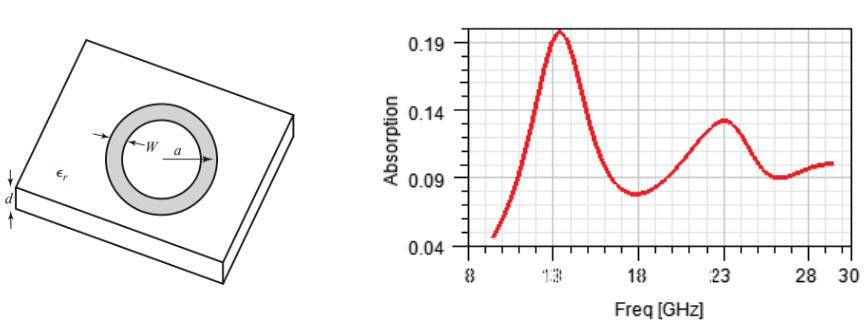
\includegraphics[width=\textwidth]{figs/todo/ring.png}
    \caption[Microstrip ring resonator.]{Microstrip ring resonator, $a=2$~mm,
    $W=0.3$~mm, $\epsilon_\text{r}=4.4$, $d=2.88$~mm, $f=11.4$~GHz. NB: no
    periodic boundary conditions! Single cell only. \part{Left} Geometry of the
    problem, from \cite{pozar2006microwave}. \part{Right} HFSS simulation
    results.}
  \label{ring}
\end{figure}

The part of the energy that is not dissipated in the conductor and substrate
losses is radiated back into space. In fact, connecting a microstrip resonator
to an active device is a space- and cost- effective way of creating an antenna.
``Microstrip antennas are planar resonant cavities that leak from their edges
and radiate.'' \cite{milligan2005modern} The ease of fabrication facilitates the
assembly of an array of such antennas, which we discuss in the following
paragraph.

\paragraph{Phased antenna arrays}

The microstrip patch antenna has a relatively wide radiation pattern on account
of its small size. Assembling an array of such antenna elements and driving it
with a fixed phase relationship between the antenna elements creates a phased
antenna array which has a response similar to a diffraction grating
(Fig.~\ref{grating}). The greater the number of antenna elements, the sharper
the peaks in the spectrum. The peak spacing in terms of wavelength is proportional
to the reciprocal antenna element spacing.

\begin{figure}[b]
   \centering
  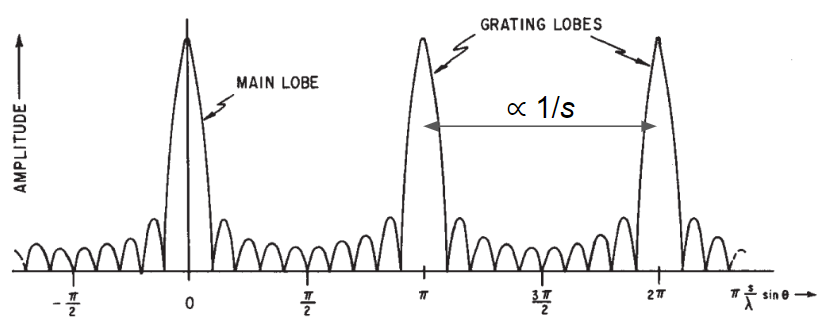
\includegraphics[width=.8\textwidth]{figs/todo/grating.png}
   \caption[Antenna array.]{Response of an antenna array as a function of element
   spacing $s$, wavelength $\lambda$, and incident angle $\theta$. Adapted from
   \cite{skolnik2008radar}.}
  \label{grating}
\end{figure}

By adjusting the phase of the signal received by each antenna element, the
antenna beam can be steered electronically. Considering a metamaterial absorber
as a phased antenna array, the phase of each element is arbitrary, therefore a
metamaterial absorber can effectively absorb energy from a wide range of angles.

\paragraph{Design process}

The key points to remember about metamaterial absorbers are that the frequency
dependence is mostly driven by the dimensions of the unit cell, as well as the
unit cell spacing. With that in mind, we can propose the following design
algorithm:

\begin{enumerate}
   \item Choose element shape and substrate material (given by
      $\epsilon_\text{r}$ and $\tan\delta$) and thickness.
   \item Tune the basic element for maximum absorption at a given frequency.
   \item Tune element spacing so grating peaks correspond to absorption peaks of
      the basic element.
   \item Tune the unit cell again, and iterate as needed.
\end{enumerate}
%
Building on this basic procedure, there are a number of design aspects to
explore:
%
\begin{itemize}
   \item Multi-frequency design (e.g., nested rings)
   \item Is it possible to invert patterns? E.g.\ a sheet with holes rather than an array of circles.
   \item What is the relative significance of ohmic vs dielectric losses? Is
      there a way to tune conductor or substrate properties to maximize
      absorption?
   \item What is the angular dependence of absorption, and to what extent is it
      relevant in a given application?
   \item What is the sensitivity to manufacturing tolerances? Is it necessary
      to experimentally determine the optimal dimensions to obtain the desired
      frequency response?
   \item What is the best way to measure the absorption of a given material?
      (E.g., use the same antenna to receive and transmit signals; have two
      separate antennas to receive and transmit, at a small angle to each other;
      use two distinct antennas but use a beam splitter to separate the forward
      and backward signals; place the metamaterial in a waveguide and measure
      absorption, etc.)
   \item Rather than using microstrip resonators, would it be better in any way
      to use other technologies, e.g.\ an array of dielectric resonators used as
      a metamaterial?
\end{itemize}
%
Rather than pursue these lines of research further, developing a good
metamaterial absorber, in the following section I consider how much of an
improvement the availability of such an absorber would be for the \CENTREX\
experiment.

\subsection{Expected effectiveness}

Literature about microwave absorbers states the effectiveness of the absorbers
in terms of an absorption coefficient for a plane wave normally incident upon an
infinite absorbing sheet. This can be further refined to study the angular
dependence, the effect of beam curvature for a Gaussian beam, the effects of the
finite size of the absorbing material, however the problem we are trying to
solve in \CENTREX\ is somewhat different. We use a beam-shaping horn in an
attempt to transmit a Gaussian beam of microwaves through a vacuum chamber.
Specifically, the beam enters through a window on one side of the chamber, and
would ideally exit the chamber through the opposing window without reflections
or scattering that would give rise to appreciable microwave power in areas
outside the main microwave beam.

In practice, the beam will get scattered from the windows, the walls of the
chamber, and the electrodes and other instrumentation present within each vacuum
chamber. The question is whether covering the interior walls of the vacuum
chamber can help cut down on the scattered radiation. One problem with this
approach is that windows form a significant part of the interior surface area
(30\%\ and 50\%\ for RC and SPA chambers, respectively). Thus a lot of the
scattered power would find its way out of the chambers, where it can get
reflected from the metallic lab equipment, and return back into the chamber
through the same windows.

To define the problem more precisely, consider Fig.~\ref{quarter} showing a
quarter of the SPA vacuum chamber. (To speed up computation, we can apply
suitable boundary conditions based on the symmetry of the problem, and need only
solve for the fields in one quarter of the volume.) The microwave beam will
enter through the window on the top and leave through the window on the bottom
of the chamber, passing between two ring-shaped electrodes (only half of one
ring shown in the figure for symmetry reasons). We desire a strong microwave
field in the central region, highlighted by the left green volume, and no
microwaves in the off-center green region to the right.

\begin{figure}
   \centering
  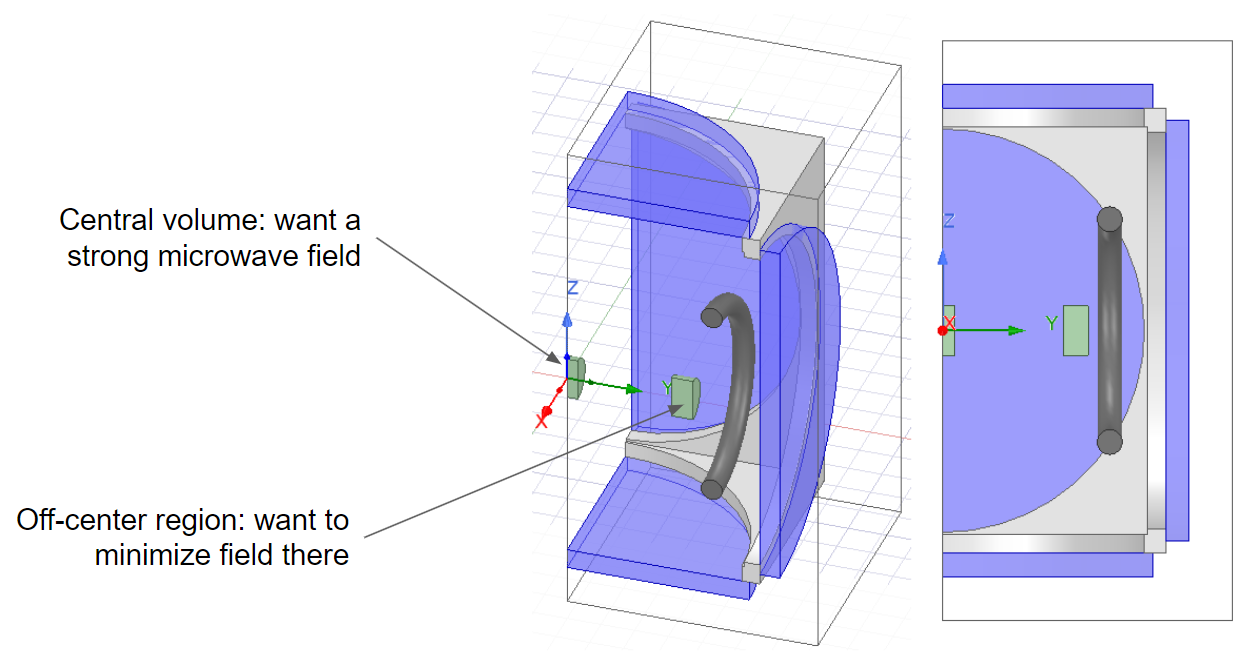
\includegraphics[width=.8\textwidth]{figs/todo/quarter.png}
    \caption[Microwaves in the SPA chamber.]{A quarter-section of the SPA vacuum
    chamber with ring electrodes.  The two green regions highlight the areas
    where we do and do not want a significant amount of microwave radiation.}
  \label{quarter}
\end{figure}

The magnitude of the microwave electric field is shown qualitatively in
Fig.~\ref{magnE} on a logarithmic scale. The simulation is repeated several
times. In the leftmost figure, only the microwave beam is included in the
simulation. In the figures to the right, various experimental features are
included in order to study their effect on scattering the microwave beam.
Qualitatively, it is obvious that the windows have the largest effect in
disturbing the beam.

In particular, observe that the presence of the vacuum chamber only contributes
minimally to the scattering. Intuitively, covering the interior walls of the
vacuum chamber with a perfect absorber would be equivalent to making the vacuum
chamber effectively disappear from the problem. However, since the chamber is
such a small contributor to the scattering, the effect of applying the absorber
appears to be negligible, even for an absolutely perfect absorber. This is borne
out by the quantitative HFSS simulation results in Table~\ref{absorbing_table},
where it is seen that the presence or absence of the vacuum chamber does not
significantly affect the scattered microwaves.

\begin{figure}
   \centering
  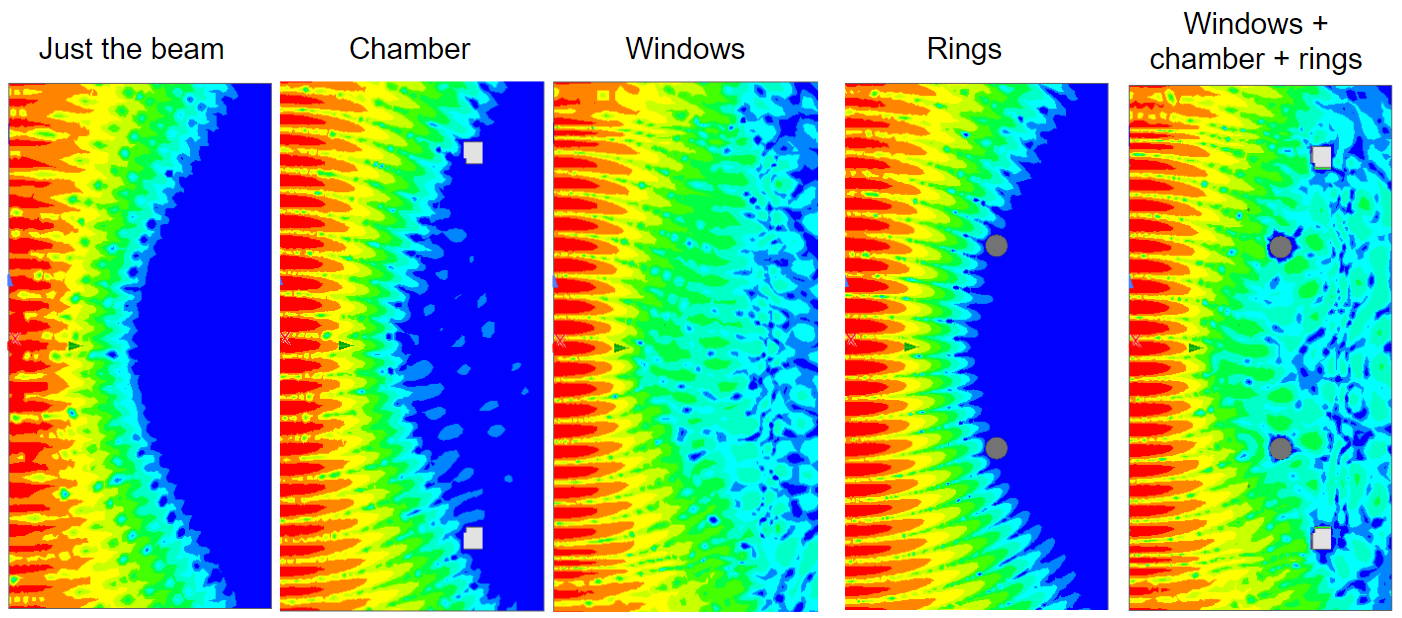
\includegraphics[width=.8\textwidth]{figs/todo/magnE.png}
    \caption[Microwaves in SPA chamber on log scale.]{Magnitude of microwave
    electric field on a log scale. For qualitative explanation only. The figures
    show half of a cut through the center of the SPA vacuum chamber.}
  \label{magnE}
\end{figure}

\begin{table*}[b]
  %\small
  \makebox[\textwidth][c]{%
    \begin{tabu} to \textwidth {rc}
      \toprule
       just the beam         & 0.10\%\\
       just chamber          & 0.09\%\\
       just windows          & 0.98\%\\
       just rings            & 0.11\%\\
       chamber + rings       & 0.11\%\\
       win + chamber         & 0.97\%\\
       win + rings           & 1.03\%\\
       win + chamber + rings & 1.02\%\\
      \bottomrule
    \end{tabu}}
    \caption[Average field magnitude vs parts of the apparatus.]{The ratio,
    expressed in percent, of the average magnitude of the electric field in the
    off-center region compared to the center region. The two regions are defined
    in Fig.~\ref{quarter}.}
    \label{absorbing_table}
\end{table*}
